Which of the following sets are domains?
\begin{teilaufgaben}
\item $\Omega=\{(x,y)\in\mathbb R^2\,|\, \text{$x$ has a real square root}\}$
\item $\Omega=\{(x,y)\in\mathbb R^2\,|\, x^2+y^2>0\}$.
\end{teilaufgaben}


\begin{loesung}
\begin{teilaufgaben}
\item
Precisely the numbers
$x\ge 0$ have a real square root, so $\Omega$ is the set
\[
\Omega=\{(x,y)\in\mathbb R^2\,|\, x\ge 0\}.
\]
This is a half plane that includes the $y$-axis.
The points on the $y$-axis are boundary points, any small neighborhood of
these points has points in $\Omega$ and points outside of it.
So $\Omega$ ist not open and therefore not a domain.
(figure \ref{20000002:fig} left).
\item
$\Omega$ consists of all points except the origin.
If $r$ is the distance of the point $(x,y)$ from $(0,0)$, then every
Ball
$B((x,y),r)$ is contained in $\Omega$, so $\Omega$ is open and therefore
a domain.
(figure \ref{20000002:fig} right).

The boundary of $\Omega$ is just the point $(0,0)$, adding this point
to $\Omega$ turns it into the plane which again is a domain.
This may be surprising at first because the common intuition is that
by adding the boundary to a domain makes it not a domain.
This indicates that one always has to go back to the definition
that domains need to be open sets.
\qedhere
\end{teilaufgaben}
\begin{figure}
\begin{center}
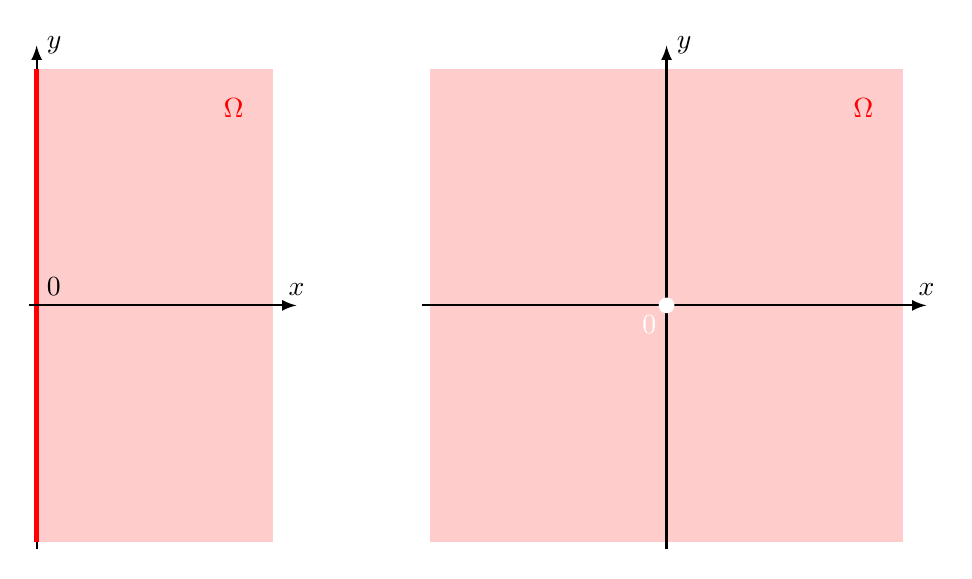
\begin{tikzpicture}[>=latex,thick]

\begin{scope}
\fill[color=red!20] (0,-3) rectangle (3,3);
\draw[->] (0,-3.1) -- (0,3.3) coordinate[label={right:$y$}];
\draw[color=red,line width=2.0pt] (0,-3) -- (0,3);
\draw[->] (-0.1,0) -- (3.3,0) coordinate[label={$x$}];
\node[color=red] at (2.5,2.5) {$\Omega$};
\node at (0,0) [above right] {$0$};
\end{scope}

\begin{scope}[xshift=8.0cm]
\fill[color=red!20] (-3,-3) rectangle (3,3);
\draw[->] (-3.1,0) -- (3.3,0) coordinate[label={$x$}];
\draw[->] (0,-3.1) -- (0,3.3) coordinate[label={right:$y$}];
\fill[color=white] (0,0) circle[radius=0.1];
\node[color=red] at (2.5,2.5) {$\Omega$};
\node[color=white] at (0,0) [below left] {$0$};
\end{scope}

\end{tikzpicture}
\end{center}
\caption{Subsets $\Omega\subset\mathbb R^2$ for problem \ref{20000002} a)
(left) 
and b) (right)\label{20000002:fig}}
\end{figure}
\end{loesung}
